\documentclass[a4paper, 12pt]{article}
% Math
\usepackage{amsmath}
\usepackage{amsthm}
\usepackage{thmtools}
\usepackage{amssymb}
\usepackage{calc}
\usepackage{bbm}

% Other packages
\usepackage{tikz}
\usepackage{geometry}
\geometry{left=2cm,right=2cm,top=2cm,bottom=2cm} 
\usepackage{graphicx}
\usepackage{enumitem}
\usepackage{listings}
\usepackage{xcolor}

\definecolor{codegreen}{rgb}{0,0.6,0}
\definecolor{codegray}{rgb}{0.5,0.5,0.5}
\definecolor{codepurple}{rgb}{0.58,0,0.82}
\definecolor{backcolour}{rgb}{0.95,0.95,0.92}

\lstdefinestyle{mystyle}{
    backgroundcolor=\color{backcolour},   
    commentstyle=\color{codegreen},
    keywordstyle=\color{magenta},
    numberstyle=\tiny\color{codegray},
    stringstyle=\color{codepurple},
    basicstyle=\ttfamily\footnotesize,
    breakatwhitespace=false,         
    breaklines=true,                 
    captionpos=b,                    
    keepspaces=true,                 
    numbers=left,                    
    numbersep=5pt,                  
    showspaces=false,                
    showstringspaces=false,
    showtabs=false,                  
    tabsize=2
}

\lstset{style=mystyle}

\usepackage{hyperref}
\hypersetup{
    colorlinks=true,
    linkcolor=blue,
    filecolor=magenta,      
    urlcolor=cyan,
}

\urlstyle{same}

% Define evironment
\theoremstyle{definition}
\newtheorem{definition}{Definition}[section]

\theoremstyle{plain}
\newtheorem{theorem}{Theorem}[section]

\theoremstyle{plain}
\newtheorem{proposition}{Proposition}[section]

\theoremstyle{plain}
\newtheorem{corollary}{Corollary}[section]

\theoremstyle{remark}
\newtheorem*{remark}{Remark}

\theoremstyle{remark}
\newtheorem{example}{Example}[section]

\newcommand{\mbb}[1]{\mathbb{#1}}
\newcommand{\mbbm}[1]{\mathbbm{#1}}
\newcommand{\mbf}[1]{\pmb{#1}}
\newcommand{\abbr}[1]{\textit{abbr.}\,\textbf{#1}}

\title{Introduction to Deep Learning}
\author{Name: Yiming MA}

\begin{document}
\maketitle
\tableofcontents
\newpage

\section{What is a Neural Network?}

Let us start with a housing price prediction example, in which there are $6$ houses, and you konw their prices and their sizes. Suppose you want to fit a function to predict the price of the houses given their sizes.

\begin{figure}[h!]
    \centering
    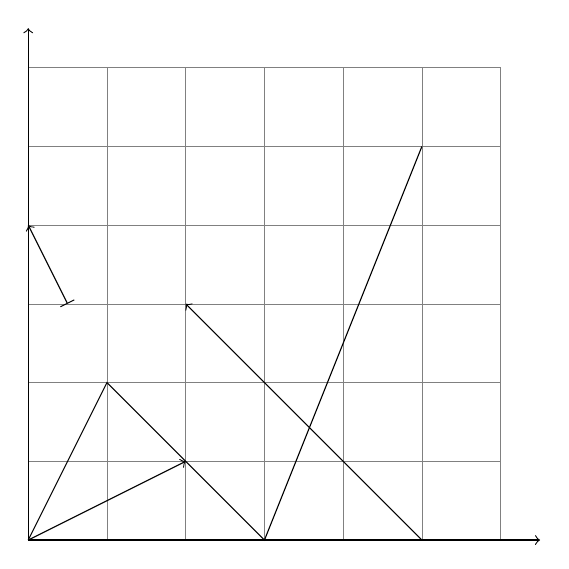
\begin{tikzpicture}[scale=1]
        \draw[help lines] (0,0) grid(6,6);
        \draw (0,0) -- (1,2)--(3,0) --(5,5);
        \draw [->] (0,0) -- (2,1);
        \draw [<-] (2,3) -- (5,0);
        \draw [|->] (0.5,3) -- (0,4);
        \draw [<->] (0,6.5) -- (0,0) -- (6.5,0); % axes
    \end{tikzpicture}
    \caption{A Test Figure}
\end{figure}


\end{document}